%% template for IEICE Transactions
%% v1.8 [2011/12/16]
\documentclass[letter]{ieice}
%\documentclass[invited]{ieice}
%\documentclass[survey]{ieice}
%\documentclass[invitedsurvey]{ieice}
%\documentclass[review]{ieice}
%\documentclass[tutorial]{ieice}
%\documentclass[letter]{ieice}
%\documentclass[brief]{ieice}
\usepackage[dvips]{graphicx}
%\usepackage[fleqn]{amsmath}
\usepackage[varg]{txfonts}
\usepackage{bm}
\usepackage{subfig}
\usepackage{array}
\usepackage{enumerate}
\usepackage{url}
\usepackage{amssymb}
\usepackage{makecell}
\usepackage{enumitem}
\setenumerate[1]{itemsep=0pt,partopsep=0pt,parsep=\parskip,topsep=5pt}
\setitemize[1]{itemsep=0pt,partopsep=0pt,parsep=\parskip,topsep=5pt}
\setdescription{itemsep=0pt,partopsep=0pt,parsep=\parskip,topsep=5pt}

\setcounter{page}{1}
%\breakauthorline{}% breaks lines after the n-th author

\field{}
%\SpecialIssue{}
%\SpecialSection{}
%\theme{}
\title{Comparing Performance of Hierarchical Identity-based Signature Schemes}
%\title[title for header]{title}
%\titlenote{}
\authorlist{% fill arguments of \authorentry, otherwise error will be caused. 
 \authorentry[chenpeixin@nudt.edu.cn]{Peixin Chen}{m}{affiliate label}
 \authorentry{Yilun Wu}{n}{affiliate label}
 \authorentry{Jinshu Su}{n}{affiliate label}[present affiliate label]
 \authorentry{Xiaofeng Wang}{n}{affiliate label}
% \authorentry{name}{membership}{affiliate label}[present affiliate label]
% \authorentry[e-mail address]{name}{membership}{affiliate label}
% \authorentry[e-mail address]{name}{membership}{affiliate label}[present affiliate label]
}
\affiliate[affiliate label]{The author is with the College of Computer, National University of Defense Technology, Changsha, 410073, China}
\paffiliate[present affiliate label]{The author is with the National Key Laboratory for Parallel and Distributed Processing, National University of Defense Technology, Changsha, 410073, China}
%\paffiliate[present affiliate label]{Presently, the author is with the }

\received{2011}{1}{1}
\revised{2011}{1}{1}
%\finalreceived{2011}{1}{1}

%% <local definitions here>

%% </local definitions here>

\begin{document}
\maketitle
\begin{summary}
Key escrow problem and high computational cost are the two major problems that hinder the widely adoption of hierarchical identity-based signature (HIBS) scheme.
HIBS schemes with either escrow-free (\emph{EF}) or online/offline (\emph{OO}) model are proposed and proved secure by Chen et al.
However, they only focus on  the formal proof of security and have not yet evaluated their schemes either theoretically or experimentally.
In this letter, several EF/OO HIBS schemes are considered. 
We study the algorithmic complexity of the schemes, and discuss the scheme performance and practicability of \emph{EF} and \emph{OO} models.
\end{summary}
\begin{keywords}
identity-based signature, computational complexity, paring based cryptography
\end{keywords}

\section{Introduction}
Identity based signature (IBS) scheme is a digital signature scheme which allows a receiver to verify message using the signer's identity as public key \cite{shamir1985identity}. 
Utilizing private key generator (PKG) to generate private key for users, Choon et al. propose the first practical IBS scheme \cite{choon2002identity}. 
Gentry et al. then present the first hierarchical IBS (HIBS) scheme, which imposes domain PKGs to reduce the workload on root PKG and solve the single-point failure problem in IBS scheme \cite{gentry2002hierarchical}. 
\par

Since the user private keys are generated by PKGs, a PKG knows the keys so that it can sign messages unscrupulously without being detected.
Such problem is referred to as key escrow problem.
Escrow-free HIBS schemes have been proposed to address the problem. 
Chen et al. propose an escrow-free model that can extent any primitive HIBS scheme to solve the key escrow problem \cite{anescrowfree2015chen}. 
They applied the model to the SHER-IBS scheme \cite{chow2004secure}, obtaining a secure scheme CWS-EF-HIBS.
\par

Besides the key escrow problem, the low computation efficiency of HIBS scheme is another concern while deploying the identity-based signature scheme.
Most IBS schemes involve computations including pairings over points on elliptic cure and point multiplications in groups, which might be too costly to be applied in lightweight devices.
Online/offline (OO) signature mechanism that divides the process of message signing into offline phase and online phase is an effective method to reduce the computational cost of signature generation \cite{even1990line}. 
Imposing the \emph{OO} mechanism, numerous identity-based online/offline signature (IBOOS) scheme have been proposed \cite{ming2010improved,chen2015ahiboos,chen2015efhiboos}. 
By extending the SHER-IBS scheme, Chen et al. propose a hierarchical IBOOS (HIBOOS) scheme with high online signing efficiency \cite{chen2015ahiboos}.
On this basis, Chen et al. propose a user-selected secret model and apply to the HIBOOS scheme to achieve an EF-HIBOOS scheme \cite{chen2015efhiboos}. 
%However, almost all of the existing work do not evaluate the performance of proposed schemes but only focus on the formal proof of security. 
They declare that the schemes they proposed are efficient enough to be practically deployed.
However, the authors have not implemented and experimental evaluated the schemes. 
\par

In this letter, we consider several HIBS schemes, which have been formally proved secure and have not yet been implemented.
The selected schemes include a primitive HIBS scheme proposed by Chow et al.  \cite{chow2004secure}, and an escrow-free extension, an online/offline extension, a comprehensive scheme proposed by Chen et al. \cite{anescrowfree2015chen,chen2015ahiboos,chen2015efhiboos}.
We implement the schemes, and evaluate the scheme performance both theoretically and experimentally. 
We analyze the evaluation results to study the signing/verification delays and transmission overhead of the schemes, as well as the performance influence of the \emph{EF} and \emph{OO} solution.

\section{Scheme Review} \label{sec-review}
In this section, we review the construction of four proved secure HIBS schemes, which we implement in this letter and evaluate in Section \ref{sec-performance}.
The schemes are primitive scheme SHER-IBS, escrow-free scheme CWS-EF-HIBS, online/offline scheme CWS-HIBOOS, and comprehensive scheme CWS-EF-HIBOOS. 

\subsection{SHER-IBS } \label{sec-sher}
Let $K$ be the security parameter given to the setup algorithm, and let $\mathcal{G}$ be a BDH parameter generator.
\\
\textbf{Setup.} The root PKG works as follows:
\begin{enumerate}
\item runs $\mathcal{G}$ on input $K$ to generate multiplicative groups $G_1, G_2$ of same prime order, and a bilinear pairing $\hat{e}: G_1 \times G_1 \rightarrow G_2$;
\item chooses random $\alpha \in \mathbb{Z}^*_p$ and two generators $g, g_2 \in G_1$, computes $g_1 = g^\alpha$;
\item randomly picks $h_1, \ldots, h_\ell \in G_1$;
\item chooses cryptographic hash functions $H: \{0, 1\}^* \times G_1 \rightarrow \mathbb{Z}_p^*$;
\item publishes $Param = \{\hat{e}, g, g_1,  g_2, h_1, \ldots, h_\ell, H\}$ as public parameters and keeps $\mathrm{MSK} = g_2^\alpha$ as master secret.
\end{enumerate}
\textbf{KeyGen.} For an input $\mathrm{ID} = \{I_1, \ldots, I_k\}$, the $level_{k-1}$ domain PKG with private key $d_{\mathrm{ID}_{\mid k-1}} = \{d'_0, \ldots, d'_{k-1}\}$ generates the key $d_\mathrm{ID}$ as follows:
\begin{enumerate}
\item picks random $r_k \in \mathbb{Z}_p^*$;
\item set $d_{\mathrm{ID}} = \{d'_0F_k(I_k)^{r_k}, d'_1, \ldots, d'_{k-1}, g^{r_k}\}$, where $F_k(x)$ $ = g_1^xh_k$.
\end{enumerate}
\textbf{Signing.} To sign a message $m$ with respect to identity $\mathrm{ID} = \{I_1, \ldots, I_k\}$, user takes the private key $d_{\mathrm{ID}} = \{d_0, d_1, \ldots, d_k\}$ as input, running the algorithm as follows:
\begin{enumerate}
\item picks a random $s \in \mathbb{Z}_p^*$ and computes $x = g_2^s$;
\item computes  $h = H(m, x)$;
\item for $j = 1, \ldots, k$, computes $y_j = d_j^{s+h}$;
\item computes $z= d_0^{s + h}$;
\item sets signature as $\sigma = \{x, y_1, \ldots, y_k, z\}$.
\end{enumerate}
\textbf{Verification.} To verify a signature $\sigma = \{x, y_1, \ldots, y_k, z\}$ on message $m$ with respect to identity $\mathrm{ID} = \{I_1, \ldots, I_k\}$, the receiver works as follows:
\begin{enumerate}
\item computes $h = H(m, x)$;
\item checks $\hat{e}(g, z) \stackrel{?}{=} \hat{e}(g_1, g_2^hx\prod_{j=1}^k y_j^{I_j})\prod_{j=1}^k \hat{e}(y_j, h_j)$.
If so, outputs 1; otherwise, outputs 0.
\end{enumerate}

\subsection{CWS-EF-HIBS } \label{sec-efhibs}
\textbf{Setup.} The root PKG works as follows:
\begin{enumerate}
\item generates groups $G_1, G_2$ and bilinear pairing $\hat{e}: G_1 \times G_1 \rightarrow G_2$;
\item chooses random $\alpha \in \mathbb{Z}^*_p$ and two generators $g, g_2 \in G_1$, computes $g_1 = g^\alpha$;
\item randomly picks $h_1, \ldots, h_\ell \in G_1$;
\item chooses cryptographic hash functions $H_1: \{0, 1\}^* \times G_1 \rightarrow \mathbb{Z}_p^*$ and $H_2: G_1 \times \{0, 1\}^* \rightarrow G_1$;
\item publishes $Param = \{\hat{e}, g, g_1,  g_2, h_1, \ldots, h_\ell, H_1, H_2\}$ as public parameters and keeps $\mathrm{MSK} = g_2^\alpha$ as master secret.
\end{enumerate}
\textbf{KeyGen.} 
The same as the \emph{KeyGen} algorithm in SHER-IBS.
\\
\textbf{Publish.} In this phase, user publishes a public parameter and gets PKG signing factor from the root PKG as follows:
\begin{enumerate}
\item randomly picks $s_{\mathrm{ID}} \in \mathbb{Z}_p^*$ as user secret and computes $g_{\mathrm{ID}} = g^{s_{\mathrm{ID}}}$;
\item publishes $g_{\mathrm{ID}}$ by submitting it to the AP;
\item sends $g_{\mathrm{ID}}$ to the root PKG, and gets $f^\alpha = H_2(g_\mathrm{ID}, \mathrm{ID})^\alpha$ computed by PKG. 
\end{enumerate}
\textbf{Signing.} User takes the private key $d_{\mathrm{ID}} = \{d_0, d_1, \ldots, d_k\}$, secret $s_{\mathrm{ID}}$ and PKG signing factor $f^\alpha$ as input, running the algorithm as follows:
\begin{enumerate}
\item picks a random $s \in \mathbb{Z}_p^*$ and computes $x = g_2^s$;
\item computes  $h = H_1(m, x)$;
\item for $j = 1, \ldots, k$, computes $y_j = d_j^{s+h}$;
\item computes $f = H_2(g_\mathrm{ID}, \mathrm{ID})$;
\item computes $z= d_0^{s + h} f^{s_\mathrm{ID}} f^\alpha = d_0^{s + h} f^{s_\mathrm{ID} + \alpha}$;
\item sets signature as $\sigma = \{x, y_1, \ldots, y_k, z, g_{\mathrm{ID}}\}$.
\end{enumerate}
\textbf{Verification.} The receiver verifies the signature as follows:
\begin{enumerate}
\item computes $h = H_1(m, x)$ and $f = H_2(g_\mathrm{ID}, \mathrm{ID})$;
\item checks whether $\hat{e}(g, z) = \hat{e}(g_1, g_2^hx \prod_{j=1}^k y_j^{I_j})\hat{e}(f, g_{\mathrm{ID}}g_1)\\ \prod_{j=1}^k \hat{e}(y_j, h_j)$ holds.
If so, outputs 1; otherwise, outputs 0.
\end{enumerate}
\textbf{Blame.} 
Given $\{\mathrm{ID}, m, \sigma\}$, where $\sigma = \{x, y_1, \ldots, y_k, z, g_{\mathrm{ID}}\}$, this algorithm requires the user parameter $g'_{\mathrm{ID}}$ with respect to the identity ID from the AP. 
It outputs 1 if and only if $g_{\mathrm{ID}} \neq g'_{\mathrm{ID}}$ and 0 otherwise.

\subsection{CWS-HIBOOS } \label{sec-hiboos}
\textbf{Setup.} 
The same as the \emph{Setup} algorithm in SHER-IBS.
\\
\textbf{KeyGen.} 
The same as the \emph{KeyGen} algorithm in SHER-IBS.
\\
\textbf{Offline Signing.} 
The signer runs the offline signing algorithm as follows:
\begin{enumerate}
\item picks a random $s \in \mathbb{Z}_p^*$ and computes $x = g_2^s$;
\item for $j = 1, \ldots, k$, computes $y_j = d_j^{s}$;
\item computes $E_{off} = \hat{e}(g_1, \prod_{j=1}^{k} d_j^{I_j})\prod_{j=1}^{k} \hat{e}(d_j, h_j)$;
\item computes $z_{off} = d_0^s$;
\item sets signature as $\sigma_{off} = \{x, y_1, \ldots, y_k, z_{off}, E_{off}\}$.
\end{enumerate}
\textbf{Online Signing.}
The signer computes the followings:
\begin{enumerate}
\item computes  $h = H(m, x)$;
\item computes $z = d_0^{h} z_{off} =  d_0^{s+h}$;
\item computes $E = E_{off}^h$;
\item sets signature as $\sigma_{on} = \{z, E\}$.
\end{enumerate}
\par
The signature is $\sigma = \{x, y_1, \ldots, y_k, z, E\}$.
\\
\textbf{Verification.} The receiver verifies the signature as follows:
\begin{enumerate}
\item computes $h = H(m, x)$;
\item checks whether the equation holds:\\
$\hat{e}(g, z) = E \cdot \hat{e}(g_1, g_2^hx\prod_{j=1}^k y_j^{I_j})\prod_{j=1}^k \hat{e}(y_j, h_j)$.\\
If so, outputs 1; otherwise, outputs 0.
\end{enumerate}
\par

\subsection{CWS-EF-HIBOOS} \label{sec-efhiboos}
\textbf{Setup.} 
The same as the \emph{Setup} algorithm in CWS-EF-HIBS.
\\
\textbf{KeyGen.} 
The same as the \emph{KeyGen} algorithm in SHER-IBS.
\\
\textbf{Publish.} User publishes a public parameter and gets PKG signing factor from the root PKG as follows:
\begin{enumerate}
\item randomly picks $s_{\mathrm{ID}} \in \mathbb{Z}_p^*$ as user secret;
\item computes $g_{\mathrm{ID}} = g^{s_{\mathrm{ID}}}$;
\item publishes $g_{\mathrm{ID}}$ by submitting it to the AP;
\item sends $g_{\mathrm{ID}}$ to the root PKG, the root PKG computes and returns $f^\alpha = H_2(g_\mathrm{ID}, \mathrm{ID})^\alpha$. 
\end{enumerate}
\textbf{Offline Signing.} 
The signer runs the offline signing algorithm as follows:
\begin{enumerate}
\item picks a random $s \in \mathbb{Z}_p^*$ and computes $x = g_2^s$;
\item for $j = 1, \ldots, k$, computes $y_j = d_j^{s}$;
\item computes $f = H_2(g_\mathrm{ID}, \mathrm{ID})$;
\item computes $E_{off} = \hat{e}(g_1, \prod_{j=1}^{k} d_j^{I_j})\prod_{j=1}^{k} \hat{e}(d_j, h_j)$;
\item computes $z_{off} = d_0^sf^{s_\mathrm{ID}} f^\alpha = d_0^sf^{s_\mathrm{ID} + \alpha}$;
\item sets the offline signature as $\sigma_{off} = \{x, y_1, \ldots, y_k, z_{off},\\ E_{off}, g_{\mathrm{ID}}\}$.
\end{enumerate}
\textbf{Online Signing.}
The signer computes the followings:
\begin{enumerate}
\item computes  $h = H_1(m, x)$;
\item computes $z = d_0^h z_{off} =  d_0^{s+h}f^{(s_\mathrm{ID} + \alpha)}$;
\item computes $E=E_{off}^h$;
\item sets signature as $\sigma_{on} = \{z, E\}$.
\end{enumerate}
\par
The signature is $\sigma = \{x, y_1, \ldots, y_k, z, E, g_{\mathrm{ID}}\}$.
\\
\textbf{Verification.} The receiver verifies the signature as follows:
\begin{enumerate}
\item computes $h = H_1(m, x)$ and $f = H_2(g_\mathrm{ID}, \mathrm{ID})$;
\item checks whether the equation holds:\\
$\hat{e}(g, z) = E\cdot \hat{e}(g_1, g_2^hx\prod_{j=1}^k y_j^{I_j})\hat{e}(f, g_\mathrm{ID}g_1)\prod_{j=1}^k \hat{e}(y_j, h_j)$.\\
If so, outputs 1. Otherwise, outputs 0.
\end{enumerate}
\textbf{Blame.} 
Given $\{\mathrm{ID}, m, \sigma = \{x, y_1, \ldots, y_k, z, g_{\mathrm{ID}}\}\}$, the algorithm requires the user parameter $g'_{\mathrm{ID}}$ with respect to the identity ID from the AP. 
It outputs 1 if and only if $g_{\mathrm{ID}} \neq g'_{\mathrm{ID}}$ and 0 otherwise.

\section{Performance Evaluation} \label{sec-performance}
%emphasize the implementation
%show the operatingg environment
In this section, we evaluate the performance of the above described schemes in terms of signing/verification computational cost and transmission overhead both theoretically and experimentally.

\subsection{Theoretically Comparison}
We make comparison of computational cost and transmission overhead between the HIBS schemes theoretically.
\par

Let $k$ denote the length of identity, $T_{e}$ the time to perform a group exponentiation computation and $T_{p}$ the time of a pairing computation.
Since the overhead of hash computation and group point multiplicative computation are negligible comparing with $T_{e}$ and $T_{p}$, we only consider these operations and neglect all the other operations.
\par

\begin{table}
\centering
\begin{footnotesize}
\caption{\label{table-performance} Algorithm computational cost. SHER stands for SHER-IBS scheme, EF for CWS-EF-HIBS scheme, OO for CWS-HIBOOS scheme, EFOO for CWS-EF-HIBOOS scheme.}
\begin{tabular}{c c c c}
\Xhline{1pt}
~ &Off. Sign &On. Sign &Verify\\
\hline
SHER &$-$ &$(k+2)T_{e}$ &$(k+1)T_{e}+(k+2)T_{p}$ \\
EF &$-$ &$(k+3)T_{e}$ &$(k+1)T_{e}+(k+3)T_{p}$ \\
OO &$(2k+2)T_{e}+2T_{p}$ &$2T_{e}$ &$(k+1)T_{e}+(k+2)T_{p}$ \\
EFOO &$(2k+3)T_{e}+(k+1)T_{p}$ &$2T_{e}$ &$(k+1)T_{e}+(k+3)T_{p}$ \\
\Xhline{1pt}
\end{tabular}
\end{footnotesize}
\end{table}

Table \ref{table-performance} shows the theoretical performance comparison. 
From the signing equation in Section \ref{sec-sher}, we can observe that the time to sign a signature in the SHER-IBS is $(k+2)T_e$, which grows linearly as the identity length $k$.
Nevertheless, with the online/offline model, the CWS-HIBOOS scheme can obtain a constant-time online signing algorithm. 
Although the scheme introduces a high computational cost offline signing algorithm, it has little influence in a real-time scenario since the algorithm is implemented offline.
Analyzing the signing/verification equation in Section \ref{sec-efhibs}, we observe that the escrow-free model only brings in a group exponentiation computation and a paring computation to the signing and verification algorithm, respectively.
It is acceptable to solve the key escrow problem.
Lowest row of Table \ref{table-performance} shows that the comprehensive scheme obtains both the benefits introduced by \emph{OO} and \emph{EF} model.
\par

\begin{table}
\centering
\begin{footnotesize}
\caption{\label{table-overhead} Transmission overhead. $k$ denotes the length of identity, size stands for the number of group elements, increased ratio is the quotient of the increased signature size divided by size of signature in SHER-IBS scheme.}
\begin{tabular}{c c c c}
\Xhline{1pt}
~ &\multicolumn{2}{c }{Signature size} &User param. size\\
\hline
SHER &$k+2$ &increased ratio &$-$ \\
\cline{2-3}
EF &$k+3$ &$1/(k+2)$ &1 \\
OO &$k+3$ &$1/(k+2)$ &$-$ \\
EFOO &$k+4$ &$2/(k+2)$ &1 \\
\Xhline{1pt}
\end{tabular}
\end{footnotesize}
\end{table}

Table \ref{table-overhead} shows the transmission overhead of the schemes.
Here, the transmission overhead includes a signature appended to an original message and a user parameter for key abusing detecting in the \emph{EF} model.
We can observe that both the \emph{EF} and \emph{OO} models introduce trivial overhead to the primitive scheme, especially when the $k$, i.e. the length of identity, is large.
\par

\subsection{Experimental Evaluation}
The evaluation results were obtained through implementations of the above four schemes based on the PBC library \cite{pbclib}.
Our implementations used the curves and parameters defined in Section \ref{sec-review} and were written in C and compiled with GCC 4.8.4 in Ubuntu 14.04. 
We ran the programs at a Desktop, which equipped Intel(R) Core Duo CPU i5-3550 at 3.30 GHz and 8G memory. 
\par

\begin{figure}[htbp]
\centering
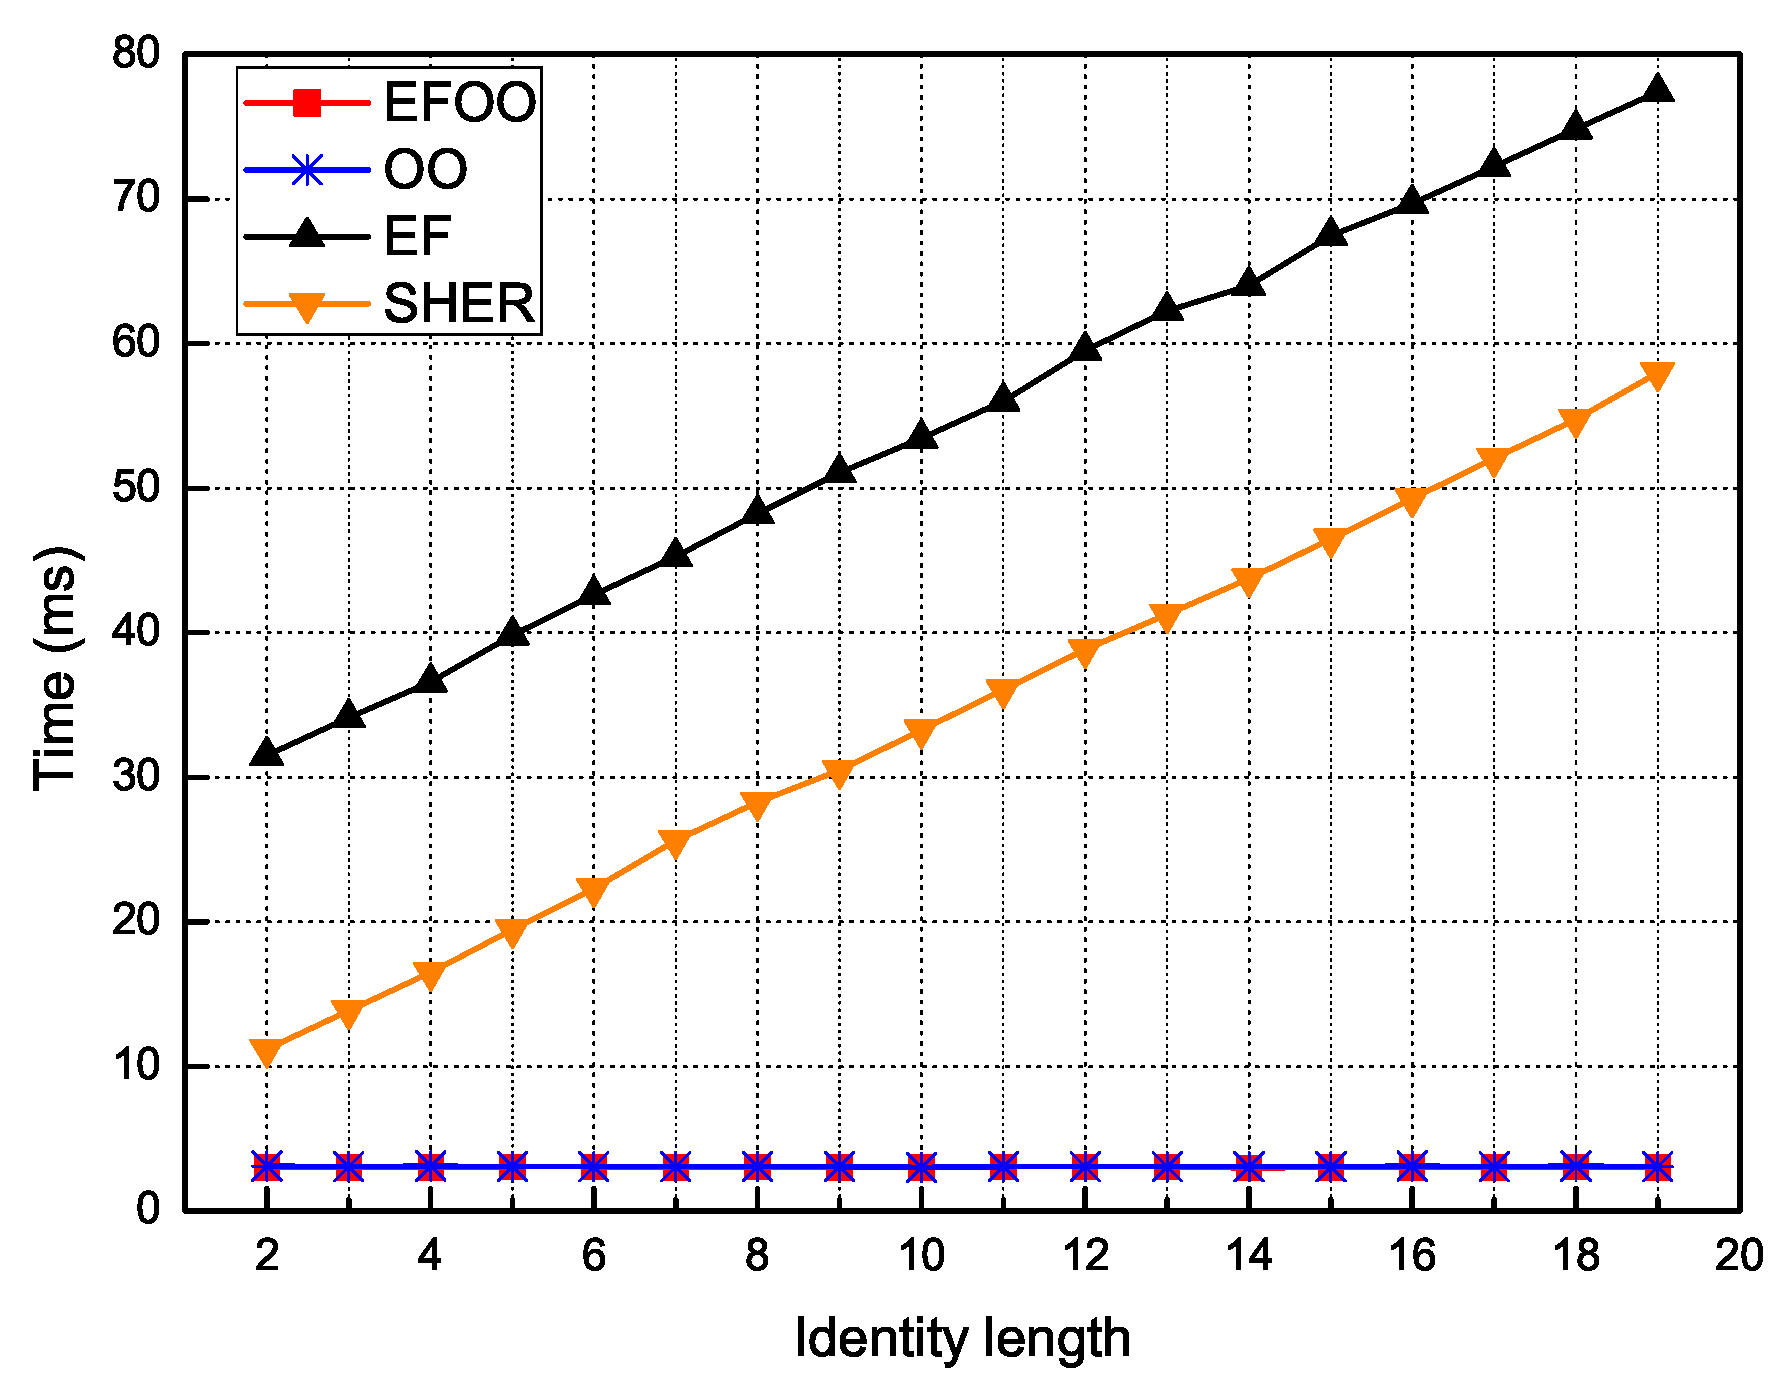
\includegraphics[width=6.6cm]{on_sign.eps}
\caption{Computational cost of online signing. Curve ``OO'' and curve ``EFOO'' are almost overlapped.} \label{fig-on-sign}
\end{figure}

Varying the length of user identity, Figure \ref{fig-on-sign} plots the computational cost of online signing of the HIBS schemes.
Note that, we take the signing procedures in SHER-IBS and CWS-EF-HIBS scheme as online signing since there are no online/offline signing procedures in the schemes.
From Figure \ref{fig-on-sign}, we can observe that the computational cost of online signing in CWS-HIBOOS and CWS-EF-HIBOOS scheme are constant, which stay around 3 ms.
On the other hand, the schemes without \emph{OO} model obtain a linear growth cost of signing.
And the lowest cost rises to 30 ms when \emph{EF} model is applied.
Thus, we find that applying the \emph{OO} model is an effective way to improve the real-time signing efficiency, especially when the \emph{EF} model has been applied.

\begin{figure}[htbp]
\centering
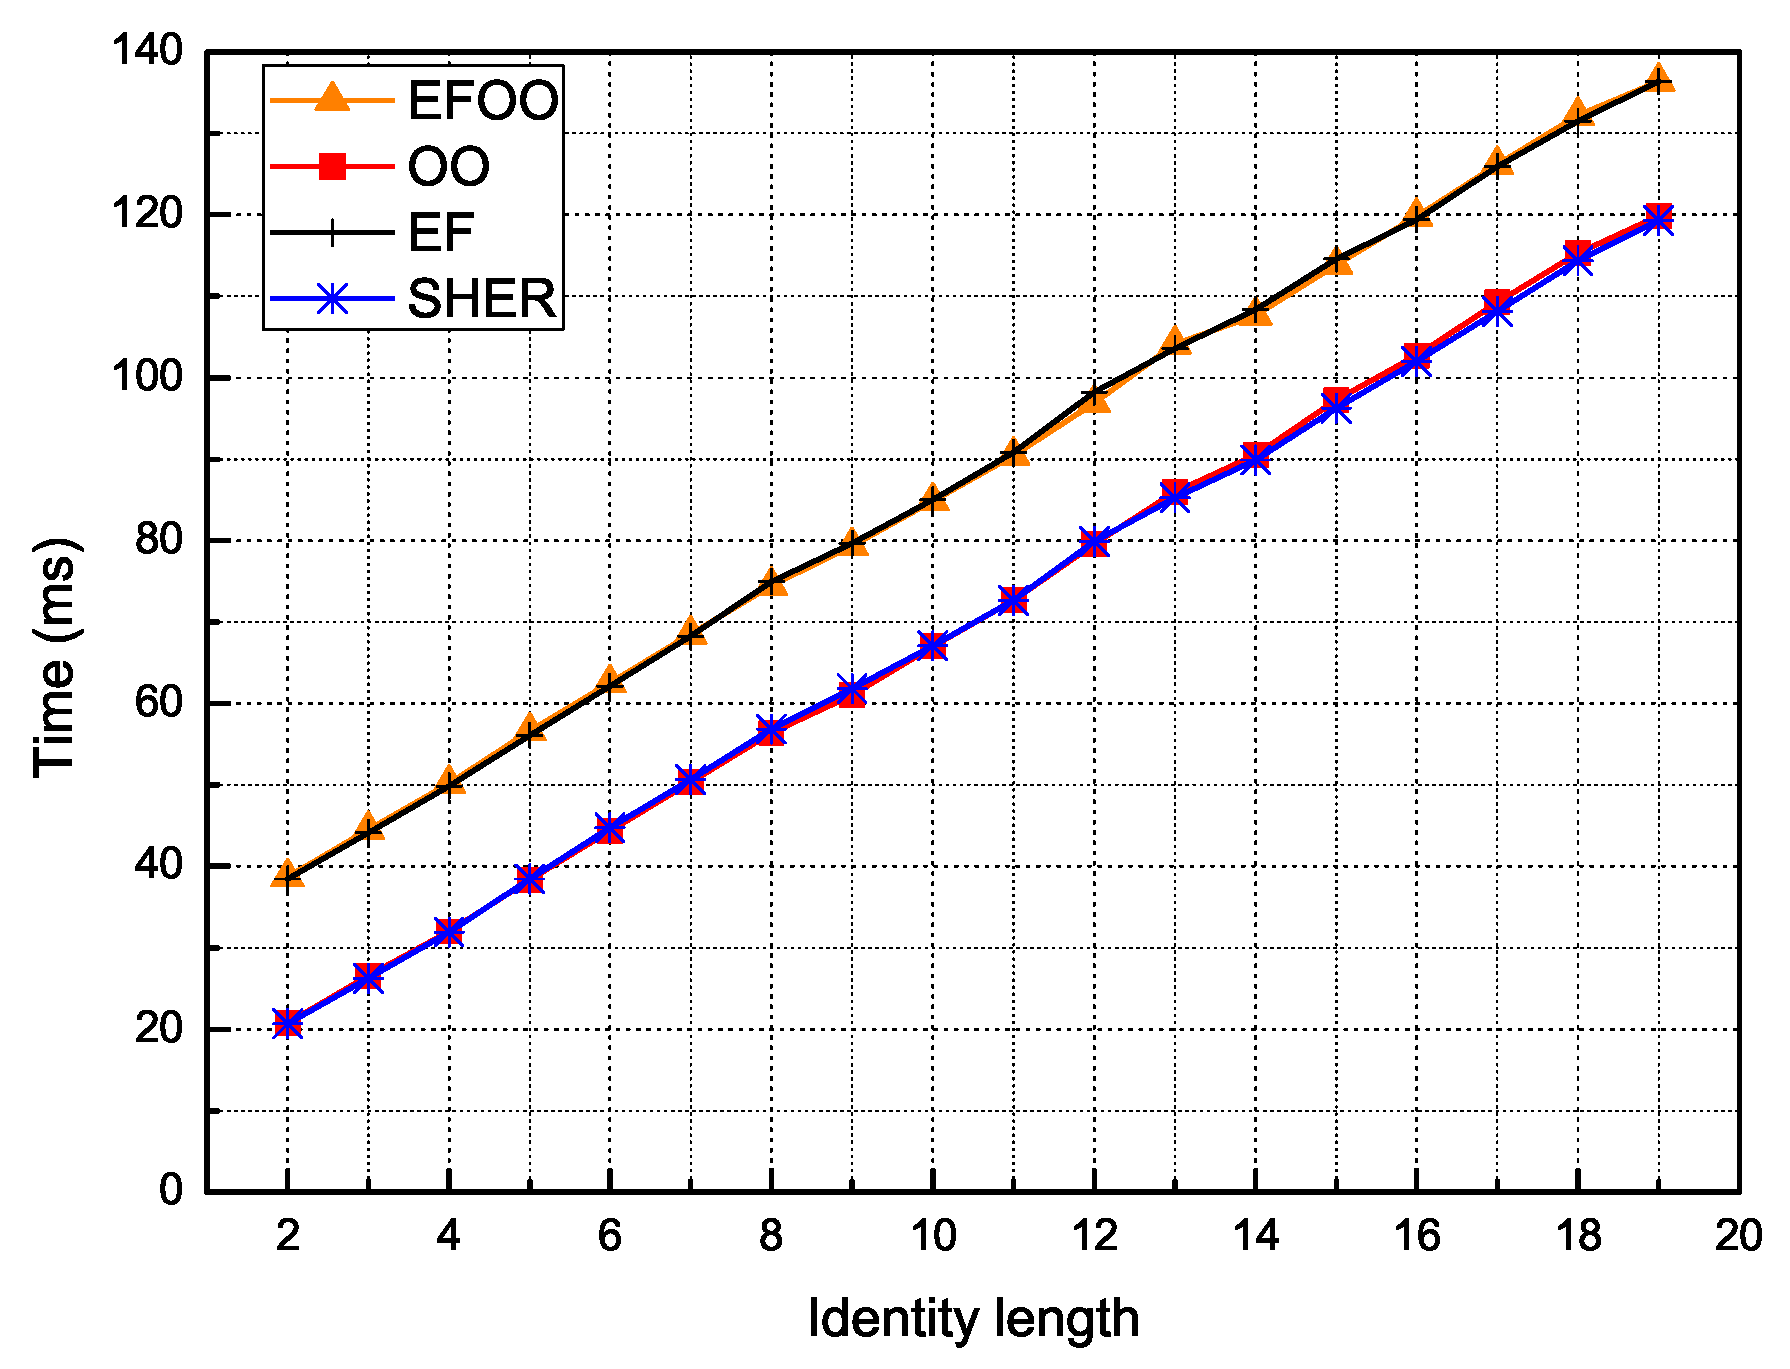
\includegraphics[width=6.7cm]{verify.eps}
\caption{Computational cost of verification. Curve ``EF'' and curve ``EFOO'' are almost overlapped, and so as the curve ``SHER'' and curve ``OO''.} \label{fig-verify}
\end{figure}

Figure \ref{fig-verify} shows the computational cost of verification of the HIBS schemes.
From the figure, we can observe that the cost of verification also grows linearly as the length of identity in each scheme, and the OO model does not improve the verification efficiency.
Comparing to online signing, the verification computational cost is still quite too high, and applying the EF model will even bring in about 20 ms to the cost. 
Therefore, we suggest that the verification algorithms need to be further improved.

\section{Conclusions}
In this work, we reviewed four HIBS schemes including a primitive scheme, an online/offline extension, an escrow-free extension and a comprehensive scheme.
We implemented the schemes and evaluated their performance in terms of signing/verification computational cost and transmission overhead  both theoretically and experimentally.
Evaluation results showed that the escrow-free model proposed by Chen et al. was an effective solution to the key escrow problem. 
And the online/offline model could improve the real-time signing efficiency. 

\section*{Acknowledgments}
This research was supported by the project of the National Science Foundation of China(NSFC) under grant no. 61303264.

\bibliographystyle{ieicetr}% bib style
\bibliography{reference}% your bib database


%\begin{thebibliography}{99}% more than 9 --> 99 / less than 10 --> 9
%\bibitem{shamir1985identity}
%A.~Shamir, Identity-based cryptosystems and signature schemes, in
%  \emph{Advances in cryptology}.\hskip 1em plus 0.5em minus 0.4em\relax
%  Springer, 1985, pp. 47--53.
%
%\bibitem{choon2002identity}
%J.~C. Choon and J.~H. Cheon, An identity-based signature from gap
%  diffie-hellman groups, \emph{Public key cryptography—PKC 2003}.\hskip
%  1em plus 0.5em minus 0.4em\relax Springer, 2002, pp. 18--30.
%  
%\bibitem{gentry2002hierarchical}
%C.~Gentry and A.~Silverberg.
%\newblock Hierarchical id-based cryptography.
%\newblock In {\em Advances in cryptology—ASIACRYPT 2002}, pages 548--566.
%  Springer, 2002.  
%
%\bibitem{anescrowfree2015chen}  
%P.~Chen, X.~Wang, and J.~Su, An Escrow-Free Hierarchical Identity-Based Signature Model for Cloud Storage, 
%\emph{Algorithms and Architectures for Parallel Processing}, Springer International Publishing, pp. 633--647, 2015.
%Springer, 2015.  
%
%\bibitem{chow2004secure}
%S.~Chow, L.~Hui, S.~Yiu, and K.~Chow, Secure hierarchical identity
%  based signature and its application, \emph{Information and Communications Security}, Springer,
%  2004, pp. 480--494.
%  
%\bibitem{even1990line}
%S.~Even, O.~Goldreich, and S.~Micali, On-line/off-line digital signatures,
%  in \emph{Advances in Cryptology—CRYPTO’89 Proceedings}.\hskip 1em plus
%  0.5em minus 0.4em\relax Springer, 1990, pp. 263--275.
%
%\bibitem{yang2013id}
%X.~Yang, C.~Li, T.~Xu, and C.~Wang, Id-based on-line/off-line
%  threshold signature scheme without bilinear pairing, \emph{Journal on
%  Communications}, vol.~8, 2013.
%
%\bibitem{chen2015ahiboos}
%P.~Chen, X.~Wang, and J.~Su, An Online/Offline HIBS Scheme for Privacy Protection of People-Centric Sensing, 
%\emph{2015 International Conference on Industrial Informatics --Computing Technology, Intelligent Technology, Industrial Information Integration (ICIICII 2015)}.
%pp.~128--131, 3--4 Dec. 2015. doi: 10.1109/ICIICII.2015.115.
%  
%\bibitem{chen2015efhiboos} 
%P.~Chen, J.~Su, B.~Zhao, X.~Wang, and I.~You, An Escrow-Free Online/Offline HIBS Scheme for Privacy Protection of People-Centric Sensing [submit],
%\emph{Security and Communication Networks}.
% 
%\bibitem{pbclib}
%B.~Lynn, The Pairing-Based Cryptography Library. Available at https://crypto.stanford.edu/pbc/
%
%\end{thebibliography}

\end{document}



\begin{table*}
\centering
\caption{\label{table-performance} Comparison of different schemes. }
\begin{tabular}{|c|c|c|c|c|c|c|}
\hline
Scheme &SHER-IBS &CWS-EF-HIBS &CWS-HIBOOS &CWS-EF-HIBOOS\\
\hline
\hline
Online/Offline Model &$\times$ &$\times$ &$\surd$ &$\surd$\\ 
\hline
Escrow-Free &$\times$ &$\surd$ &$\times$ &$\surd$\\
\hline
\hline
Offline Sign. Comp. Cost &$-$ &$-$ &$(2k+2)E+2P$ &$(2k+3)E+(k+1)P$\\
\hline
Online Sign. Comp. Cost &$(k+2)E$ &$(k+3)E$ &$2E$ &$2E$\\
\hline
Verify Comp. Cost &$(k+1)E+(k+2)P$ &$(k+1)E+(k+3)P$ &$(k+1)E+(k+2)P$ &$(k+1)E+(k+3)P$\\
\hline
\hline
Private key Size & & & &\\
\hline
Signature Size & & & &\\
\hline
\end{tabular}
\end{table*}



%\begin{figure*}[htbp]
%\centering
%\subfloat[online signing]{
%\label{fig-on-sign}
%\begin{minipage}[t]{0.45\textwidth}
%\centering
%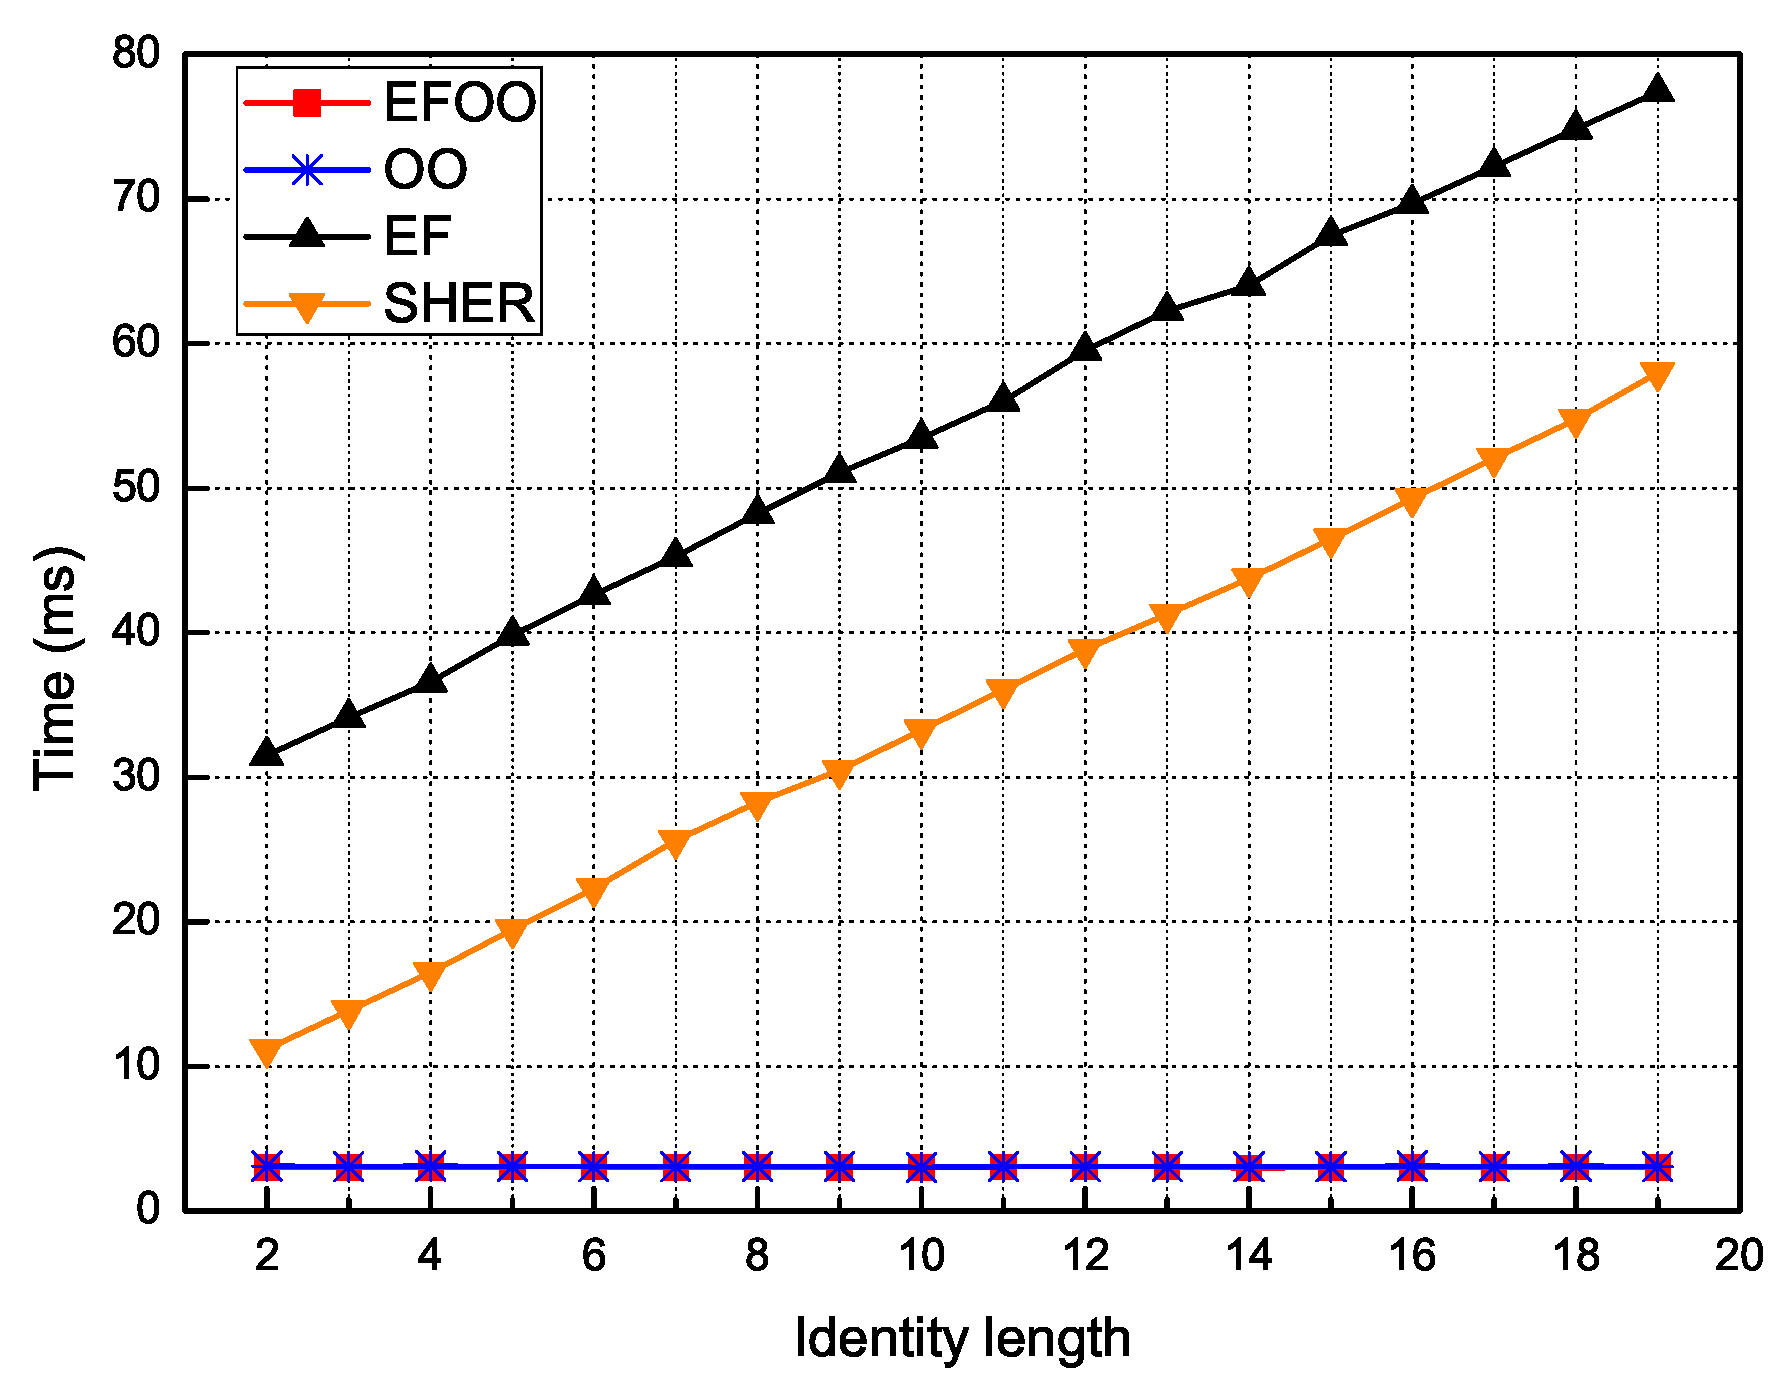
\includegraphics[width=7cm]{on_sign.eps}
%\end{minipage}
%}
%\subfloat[verification]{
%\label{fig-verify}
%\begin{minipage}[t]{0.45\textwidth}
%\centering
%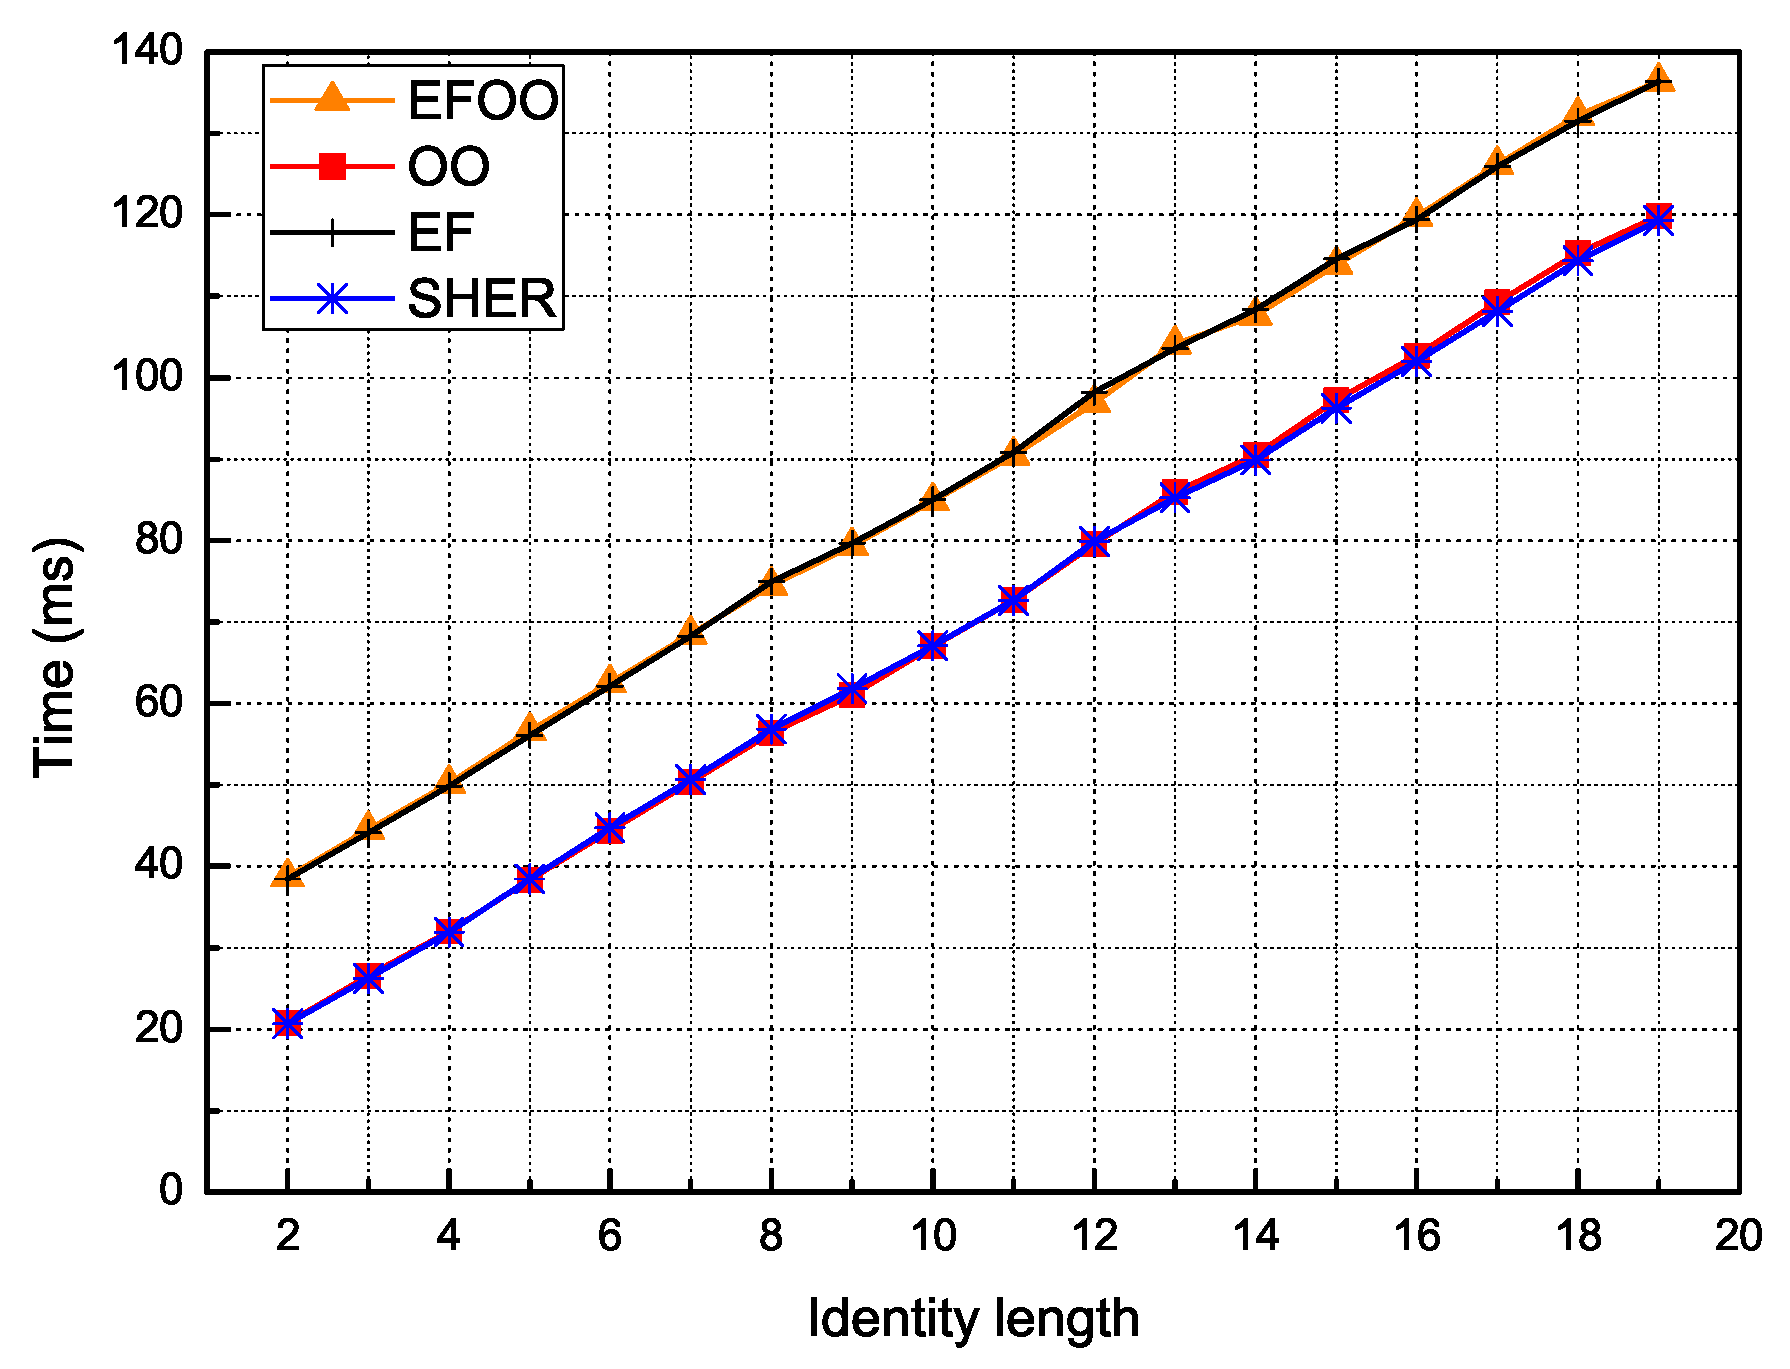
\includegraphics[width=7cm]{verify.eps}
%\end{minipage}
%}
%\caption{Computational cost} \label{fig-comcost}
%\end{figure*}



%The motivation scheme and first scheme achieve the constant size signatures. But the private keys rely on the users identity. So they can not apply to the large scale networks. Our main construction solves this limitation. The new scheme achieves constant size private keys and signatures. It is more efficient than the existing works. In addition, e(g,g)  can be precomputed. Hence there are 3 pairing computations in the verification algorithm. 